\documentclass[12pt]{article}
%% arXiv paper template by Flip Tanedo
%% last updated: Dec 2016



%%%%%%%%%%%%%%%%%%%%%%%%%%%%%
%%%  THE USUAL PACKAGES  %%%%
%%%%%%%%%%%%%%%%%%%%%%%%%%%%%

\usepackage{amsmath}
\usepackage{amssymb}
\usepackage{amsfonts}
\usepackage{graphicx}
\usepackage{xcolor}
\usepackage{nopageno}
\usepackage{enumerate}
\usepackage{parskip}
\usepackage{framed}
%\usepackage{bbm} 


\renewcommand{\thesection}{}
\renewcommand{\thesubsection}{\arabic{subsection}}

%%%%%%%%%%%%%%%%%%%%%%%%%%%%%%%%%%%%%%%%%%%%%%%
%%%  PAGE FORMATTING and (RE)NEW COMMANDS  %%%%
%%%%%%%%%%%%%%%%%%%%%%%%%%%%%%%%%%%%%%%%%%%%%%%

\usepackage[margin=2cm]{geometry}   % reasonable margins

\graphicspath{{figures/}}	        % set directory for figures

% for capitalized things
\newcommand{\acro}[1]{\textsc{\MakeLowercase{#1}}}    

%\numberwithin{equation}{section}    % set equation numbering
\renewcommand{\tilde}{\widetilde}   % tilde over characters
%\renewcommand{\vec}[1]{\mathbf{#1}} % vectors are boldface

\newcommand{\dbar}{d\mkern-6mu\mathchar'26}    % for d/2pi
\newcommand{\ket}[1]{\left|#1\right\rangle}    % <#1|
\newcommand{\bra}[1]{\left\langle#1\right|}    % |#1>
\newcommand{\Xmark}{\text{\sffamily X}}        % cross out

\let\olditemize\itemize
\renewcommand{\itemize}{
  \olditemize
  \setlength{\itemsep}{1pt}
  \setlength{\parskip}{0pt}
  \setlength{\parsep}{0pt}
}


% Commands for temporary comments
\newcommand{\comment}[2]{\textcolor{red}{[\textbf{#1} #2]}}
\newcommand{\flip}[1]{{\color{red} [\textbf{Flip}: {#1}]}}
\newcommand{\email}[1]{\texttt{\href{mailto:#1}{#1}}}

\newenvironment{institutions}[1][2em]{\begin{list}{}{\setlength\leftmargin{#1}\setlength\rightmargin{#1}}\item[]}{\end{list}}


\usepackage{fancyhdr}		% to put preprint number



% Commands for listings package
%\usepackage{listings}      % \begin{lstlisting}, for code
%
% \lstset{basicstyle=\ttfamily\footnotesize,breaklines=true}
%    sets style to small true-type



%%%%%%%%%%%%%%%%%%%
%%%  HYPERREF  %%%%
%%%%%%%%%%%%%%%%%%%

%% This package has to be at the end; can lead to conflicts
\usepackage{microtype}
\usepackage[
	colorlinks=true,
	citecolor=black,
	linkcolor=black,
	urlcolor=green!50!black,
	hypertexnames=false]{hyperref}





\begin{document}


\begin{center}

    {\Large \textsc{Long HW 3}:
    \textbf{Symmetries}}
    
\end{center}

\vskip .4cm

\noindent
\begin{tabular*}{\textwidth}{rl}
	\textsc{Course:}& Physics 165, \emph{Introduction to Particle Physics} (2018)
	\\
	\textsc{Instructor:}& Prof. Flip Tanedo (\email{flip.tanedo@ucr.edu})
	\\
	\textsc{Due by:}& \textbf{Tuesday}, January 30
\end{tabular*}

\noindent
This is the main weekly homework set. Unless otherwise stated, give all responses in natural units where $c = \hbar = 1$ and energy is measured in electron volts (usually MeV or GeV). 

\flip{1/27: Corrected sign error in (19), thanks Adam G.}


\subsection{U(1) symmetries}


\begin{framed}
\textbf{Background}.	
Thus far, our model building rules have been the following:
\begin{enumerate}
	\item Remember the spacetime symmetries that we'll assume for all of our theories: Translation symmetry imposes 4-momentum conservation. Lorentz symmetry enforces spin indices (e.g.\ $\alpha$, $\dot\beta$, $\mu$).
	\item Specify any additional \textbf{internal symmetries}. These symmetries have different \textbf{representations}, which means that the particles that transform under these symmetries will have their own indices. Each type of representation (each type of index) comes with a list of invariant tensors: the metric, the unit matrix, and at least one object that relates different kinds of indices.
	\item List your particles and identify what indices they have. 
	\item Write down the 3-particle\footnote{The two-point vertices just define particles. Higher-point vertices are allowed, but we will see that there are reasons not to worry about them too much.} vertices that are allowed. A vertex is allowed if you can use invariant tensors to contract all indices.
\end{enumerate}
The kinds of internal symmetries that give you indices are called \textbf{non-Abelian} symmetries. In class we looked at a non-Abelian symmetry called SU(2). Remember that this is a symmetry where the simplest representation came with two particles, $D^a = (D^1, D^2)$.  Later we will also consider the symmetry SU(3), whose simplest representation has three particles: $F = (F^1, F^2, F^3)$. You can guess that SU($N$) has a simplest representation with $N$ particles. This funny name means the \textbf{special unitary} group of $N\times N$ matrices. There are other kinds of non-Abelian groups with similarly silly names.

Thus far we haven't said anything about electric charge. This comes from what is called an \textbf{Abelian} symmetry. Unlike the non-Abelian symmetries, an Abelian symmetry does \emph{not} come with indices. Instead, Abelian symmetries are \emph{complex phases}. Here's how it works: a particle $\psi$ with charge $q$ transforms under a phase $\theta$ by
\begin{align}
	\psi \to e^{iq\theta} \psi \ .
	\label{eq:phase}
\end{align}
The anti-particle transforms with the opposite phase:
\begin{align}
	\psi^\dag \to \left(e^{iq\theta}\psi\right)^\dag = e^{-iq\theta}\psi^\dag \ .
\end{align}
Abelian symmetries called U(1) symmetries, short for ``unitary $1\times 1$ matrix,'' which you may realize is an exceedingly fancy way of saying a complex phase.
\end{framed}

Let's make up a theory that has nothing to do with the real universe. This not-the-real-universe model has the same spacetime symmetries (translation, Lorentz), but none of the internal symmetries of the real universe. 
%
Now let's imagine that this universe has one Abelian internal symmetry that we're going to call \emph{megacharge}.  Let's populate this universe with three types of scalar particles: $X$, $Y$, and $Z$. These have megacharge 1, 2, and 3 respectively. Recall that this means that their anti-particles have negative megacharge, for example $Y^\dag$ has megacharge $-2$. 

\subsubsection{Rules of the $XYZ$ theory}

Draw the allowed three-particle Feynman rules between the $X$, $Y$, $Z$ and their antiparticles. 

\textsc{Remark}: Because these are scalar particles, you don't have to worry about Lorentz indices (yay). You just have to write down products of three particles that conserve charge. I think there are four total. 

\subsubsection{Ultracharge}

Suppose that \emph{in addition} to megacharge, our hypothetical universe \emph{also} has a different U(1) symmetry that we'll call \emph{ultracharge}. Suppose that the charge assignments are as follows:
\begin{center}
\begin{tabular}{|l|c|c|}
\hline
    & Megacharge & Ultracharge \\ \hline
$X$ & $1$        & $2$        \\ \hline
$Y$ & $2$        & $1$        \\ \hline
$Z$ & $3$        & $3$        \\ \hline
\end{tabular}
\end{center}
Which 3-particle Feynman rule(s), if any, are still valid? Valid Feynman rules are those which combine three particles in a way that is invariant under both megacharge and ultracharge. 

\textsc{Remark}: to be clear, suppose a particle $\psi$ has megacharge $q_m$ and ultracharge $q_u$. We can then do a megacharge transformation by a parameter $\theta_m$ that we get to choose to be anything, and similarly an ultracharge transformation by a parameter $\theta_u$ that we get to choose to be anything. The particle transforms as:
\begin{align}
	\psi \to e^{iq_m\theta_m} e^{iq_u\theta_u} \psi \ .
\end{align}


\subsubsection{(mega+ultra)charge and (mega-ultra)charge}

Here's something neat about symmetries: you can take linear combinations of them and they're still symmetries. Consider the following two symmetries: $(M+U)$ and $(M-U)$. A particle with megacharge $q_m$ and ultracharge $q_u$ has charges
\begin{align}
	q_{m+u} &= q_m + q_u
	&
	q_{m-u} &= q_m - q_u \ ,
\end{align}
under $(M+U)$ and $(M-U)$ respectively. Now suppose I imagine a new universe that doesn't know anything about megacharge or ultracharge, but only knows about $(M+U)$ charge and $(M-U)$ charge. Introduce the $X$, $Y$, and $Z$ particles with the following charges:
\begin{center}
\begin{tabular}{|l|c|c|}
\hline
    & $(M+U)$ & $(M-U)$ \\ \hline
$X$ & $3$        & $-1$        \\ \hline
$Y$ & $3$        & $1$        \\ \hline
$Z$ & $6$        & $0$        \\ \hline
\end{tabular}
\end{center}
What three-particle Feynman rules are allowed?


\subsection{The Yukawa interaction, again}

In your short homework this week, you explored a simple theory of spin-1/2 particles interacting with a spin-0 particle. We re-introduce that theory here. The theory has an SU(2) symmetry with doublet indices $a,b,c,\cdots \in \{1,2\}$ and triplet indices $A,B,\cdots \in \{1,2,3\}$. You have the following tensors:

\begin{itemize}
	\item {Lorentz metrics}: metric for vectors ($\eta^{\mu\nu}$, $\eta_{\mu\nu}$), metric for spinors ($\varepsilon^{\alpha\beta}$, $\varepsilon_{\alpha\beta}$, $\varepsilon^{\dot\alpha\dot\beta}$, $\varepsilon_{\dot\alpha\dot\beta}$)
	\item {Lorentz tensor}: $\sigma$-matrices ($\sigma^{\mu}_{\phantom\mu \alpha\dot\beta}$)
	\item SU(2) metrics: $\epsilon_{ab}$, $\epsilon^{ab}$, $\delta_{AB}$ (i.e.\ you can contract two upper $A$ indices)
	\item SU(2) tensors: $f^{abc}$, $T^{Aa}_{\phantom{Aa}b}$
	\item The identity: $\delta^a_b$, $\delta^\alpha_\beta$, etc.
	\item Momenta: $p^\mu$ of any particle going into the vertex
\end{itemize}

You have the following particles:
\begin{center}
	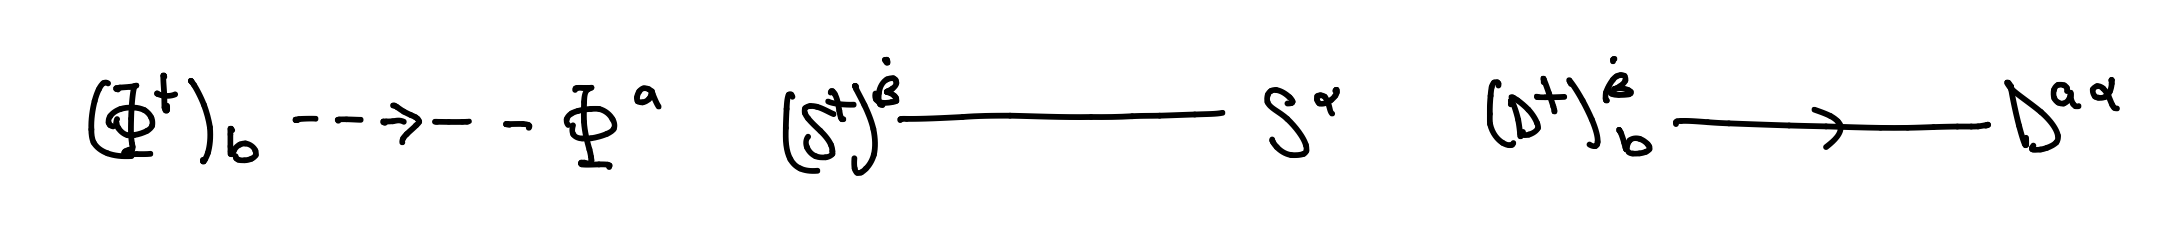
\includegraphics[width=.7\textwidth]{HW3a.png}
\end{center}
Here $\Phi^a$ is an SU(2) doublet, meaning it has two components. It has an anti-particle, $(\Phi^\dag)_b$. Observe that $\Phi$ is a Lorentz scalar: it doesn't have any spinor or vector index. The particle $S$ is a spin-1/2 particle that is an SU(2) singlet (``SU(2) scalar''), it has a spinor index but does not have any SU(2) indices. It has an antiparticle $(S^\dag)^{\dot \beta}$ The particle $D$ is an SU(2) doublet and a spin-1/2 particle with spinor indices. It has an anti-particle $(D^\dag)^{\dot \beta}_{\phantom\beta b}$.


You found that you could write the following Feynman rules:
%\begin{center}
\begin{align}
	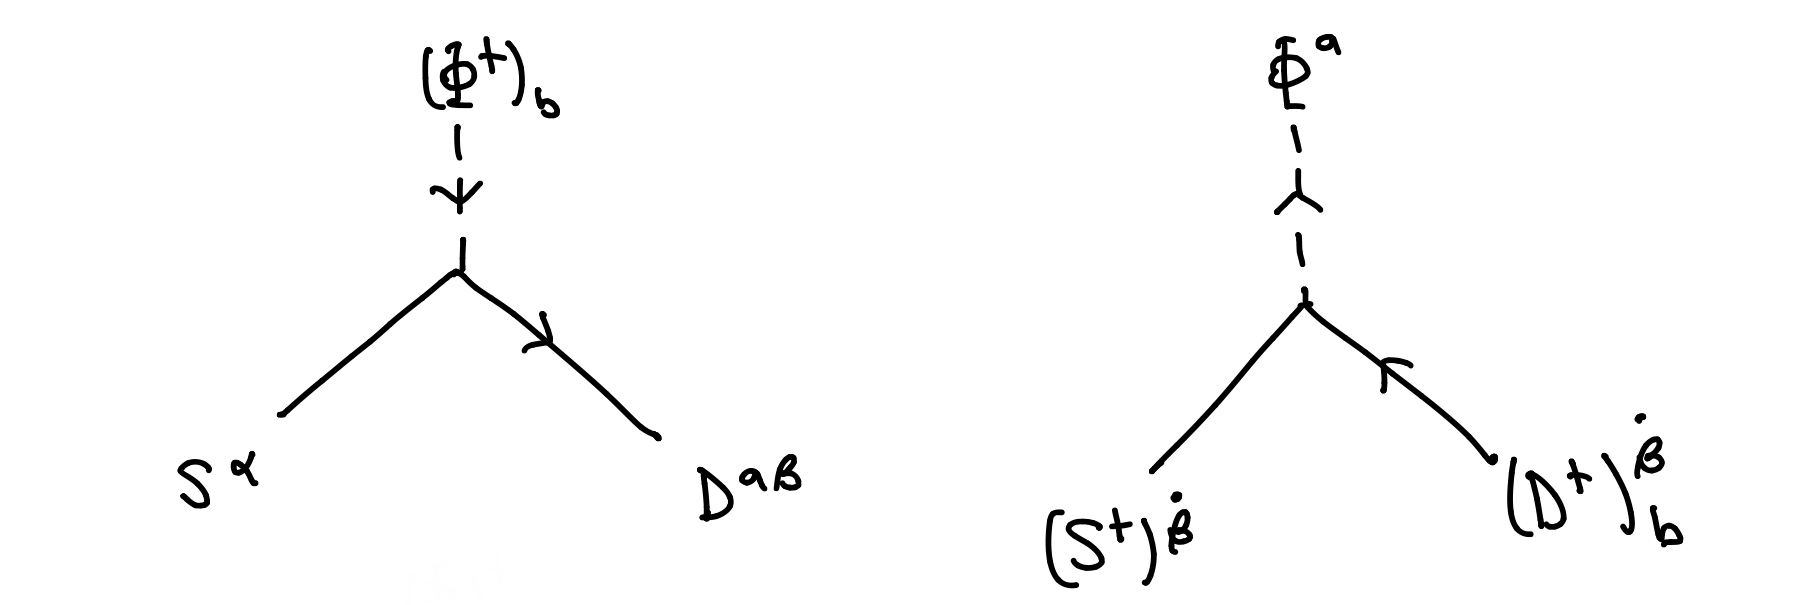
\includegraphics[width=.5\textwidth]{HW3aa.png}
	\label{eq:old:rules}
\end{align}
%\end{center}
%That is, for each proposed Feynman rule, write down an invariant using the tensors above and the particles. For example,  your answer for the first diagram should look like:
%\begin{align*}
%	S^\alpha (\Phi^\dag)_b D^{a\beta} \left[\text{some combination of tensors}\right]^{b}_{\phantom{b}\alpha\beta a}
%\end{align*}


\subsubsection{A weird Feynman rule}

Show that the following is an allowed Feynman rule:
%\begin{center}
\begin{align}
	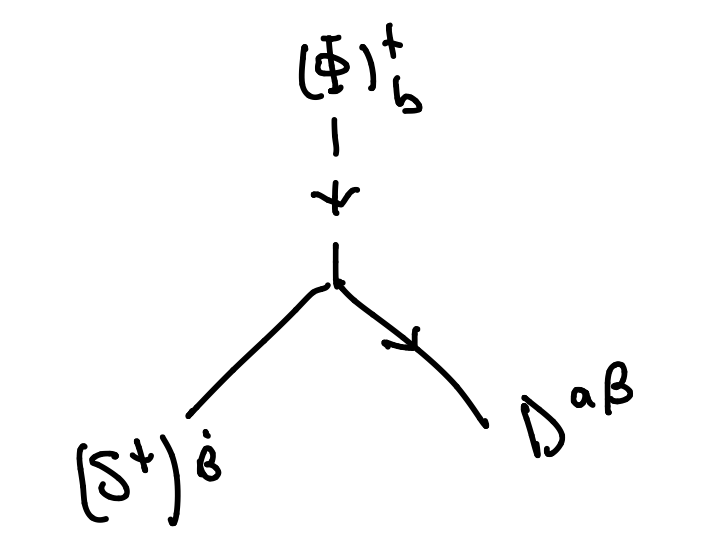
\includegraphics[width=.3\textwidth]{HW3aaa.png}
\label{eq:weird:rule}	
\end{align}
Observe that the structure of this interaction is very different from the previous two rules. You may have to use the momentum four-vector as an available tensor\footnote{Each line has an associated momentum. Determining \emph{which} combination of momenta to use is tricky and we won't dwell on it. You can just write $p_\mu$ as some general momentum.}. 

\subsubsection{Adding electric charge}

Now suppose in addition to all the indices we've listed, let's assign `electric' charge to our particles:
\begin{itemize}
	\item The $D$ particle has electric charge $+1$. This means that $D^\dag$ has electric charge $-1$.
	\item $\Phi$ has no electric charge.
	\item $S$ has electric charge $q$ and so $S^\dag$ has electric charge $-q$.
\end{itemize}
What value of $q$ permits the rules in  (\ref{eq:old:rules}) but prohibits the weird rule in (\ref{eq:weird:rule})?

\textsc{Remark}: A theory with more symmetries is more constrained. We see that imposing electromagnetic symmetry reduces the number of possible Feynman rules in the theory.



\subsection{A U(1) subgroup of SU(2)}

The internal symmetry SU(2) has three elements. This means that there are three `rotation' axes in this abstract space. This is similar (and intimately related to) the rotations of ordinary three-dimensional space. In contrast to the U(1) symmetry, where there is only one type of rotation (rephasing). In other words: for SU(2), you have to specify three rotation angles to define a transformation.

In class we met the \textbf{doublet} representation, $D^a$ where $a=1,2$. A more general name for this is the \textbf{fundamental} representation---the name indicates that this is somehow the intuitive object that you'd want to rotate. This is similar to how 3-vectors are the intuitive object that you'd want to rotate in real space\footnote{To describing rotational symmetry, you'd start with $R^i_{\phantom i j} v^j$, not ``here's how a matrix transforms.''}. The objects that define rotations are the tensors that we called $(T^A)^a_{\phantom a b}$. The index $A$, which we said is also related to the \textbf{triplet} (fancy name: \textbf{adjoint}) representation, is related to the three rotation axes. You probably already know them:
\begin{align}
	(T^1)^a_{\phantom a b} &= \frac 12 (\sigma^1)^a_{\phantom a b} =
	\frac 12
	\begin{pmatrix}
		0 & 1 \\
		1 & 0
	\end{pmatrix}
	\\
	(T^2)^a_{\phantom a b} &= \frac 12 (\sigma^2)^a_{\phantom a b} =
	\frac 12
	\begin{pmatrix}
		0 & -i \\
		i & 0
	\end{pmatrix}
	\\
	(T^3)^a_{\phantom a b} &= \frac 12 (\sigma^3)^a_{\phantom a b} =
	\frac 12
	\begin{pmatrix}
		1 & 0 \\
		0 & -1
	\end{pmatrix} \ .
\end{align}
If you rotate by $\theta_1$ about the $T^1$ axis in the internal space, then the particles in a doublet rotate into each other as follows:
\begin{align}
		D^a & \to \exp\left[i\theta_1 (T^1)^a_{\phantom{a}b}\right]
		D^b
		&
		\text{or}&
		&
	\begin{pmatrix}
		D^1 \\
		D^2
	\end{pmatrix}
	\to 
	\exp\left[\frac{i\theta_1}2
	\begin{pmatrix}
		0 & 1 \\
		1 & 0
	\end{pmatrix}\right]
	\begin{pmatrix}
		D^1 \\
		D^2
	\end{pmatrix} \ .
\end{align}
The matrix exponential is defined by its Taylor expansion. For small $\theta$, you can just take the first few terms and see that the $D^1$ and $D^2$ particles mix into one another. 

It's much easier to examine the effect of a rotation about the $T^3$ axis. Show that the components of $D$ transform as a phase under a rotation about this axis. That is, perform a $T^3$ axis rotation by some angle, $\theta_3$. Write explicitly how $D^1$ and $D^2$ transform. Compare this to (\ref{eq:phase}). Comment on how it looks like $T^3$ is related to some kind of \emph{Abelian} symmetry; what are the charges of $D^1$ and $D^2$ under this Abelian symmetry?

\textsc{Hint}: If you are unfamiliar with matrix exponentiation (it shows up all the time in quantum mechanics), then it's useful to know that
\begin{align}
	\exp\begin{pmatrix}
		A & 0 \\
		0 & B
	\end{pmatrix}
	=
	\begin{pmatrix}
		e^A & 0  \\
		0 & e^B
	\end{pmatrix} \ .
\end{align}

\textsc{Remark}: In problem 1 we talked about multiple U(1) symmetries that mix. In this problem, we found something that looks like a U(1) symmetry ``inside'' SU(2). Both of these problems worked with `toy' theories that are not models of our universe. However, the \emph{critical} piece of the Standard Model has to do with how an ordinary U(1) symmetry (which is called hypercharge) mixes with a U(1) inside an SU(2) symmetry. This will give rise to the photon and the $Z$ boson. The two `leftover' symmetry axes in the SU(2) will be identified with the $W^\pm$. 

%\subsection{The SU(2) charge of SU(2) gauge bosons}


\vspace{1em}
\appendix
{\Large\textbf{Extra credit}}
%\vspace{-1em}

\subsection{How spinors transform}

What is the difference between left-handed and right-handed spinors? Both types spinors pick up a minus sign after doing a $2\pi$ rotation about the quantization axis. They differ in how they get there. 

Here's what you need to know. Our notation may be slightly different from class. You have the following tensors:
\begin{align}
	\left(\sigma^\mu\right)_{\alpha\dot\beta}
	&=
	\left[
	\begin{pmatrix}
		 1 &  0\\
		 0 &  1
	\end{pmatrix}\ , \;
	\begin{pmatrix}
		 0 &  1\\
		 1 &  0
	\end{pmatrix}\ , \;
	\begin{pmatrix}
		 0 & -i\\
		 i &  0
	\end{pmatrix}\ , \;
	\begin{pmatrix}
		 1 &  0\\
		 0 & -1
	\end{pmatrix}
	\right]
	\\
	\left(\bar\sigma^\mu\right)^{\dot\alpha\beta}
	&=
	\left[
	\begin{pmatrix}
		 1 &  0\\
		 0 &  1
	\end{pmatrix}\ , \;
	\begin{pmatrix}
		 0 & -1\\
		-1 &  0
	\end{pmatrix}\ , \;
	\begin{pmatrix}
		 0 &  i\\
		-i &  0
	\end{pmatrix}\ , \;
	\begin{pmatrix}
		-1 &  0\\
		 0 &  1
	\end{pmatrix}
	\right] \ .
\end{align}
Thus $\sigma^0$ and $\bar\sigma^0$ are both the identity matrix, but with different index structure. A convenient way to remember this is:
\begin{align}
	\sigma^\mu &= ({1}_{2\times 2}, \vec{\sigma})
	&
	\bar\sigma^\mu &= ({1}_{2\times 2}, -\vec{\sigma}) \ .
\end{align}
These are objects that convert between vector ($\mu$), right-handed ($\dot\alpha$), and left-handed ($\alpha$) indices. The theory of Lorentz symmetry tells us that the objects that \emph{generate Lorentz transformations}\footnote{I use the term `generate' deliberately, it may sound familiar from quantum mechanics where you have \textbf{generators} of certain transformations.} are the following:
\begin{align}
	\left(\sigma^{\mu\nu}\right)_\alpha^{\phantom\alpha \beta}
	&= 
	\frac 14 \left(\sigma^\mu \bar\sigma^\nu - \sigma^\nu\bar\sigma^\mu\right)_{\alpha}^{\phantom\alpha \beta} 
	\\
	\left(\bar\sigma^{\mu\nu}\right)^{\dot\alpha}_{\phantom\alpha \dot\beta}
	&= 
	\frac 14 \left(\bar\sigma^\mu \sigma^\nu - \bar\sigma^\nu \sigma^\mu\right)^{\dot\alpha}_{\phantom\alpha \dot\beta} \ .
\end{align}
For example (and here I'm doing most of the hard work for you):
\begin{align}
	\left(\sigma^{03}\right)_\alpha^{\phantom\alpha \beta}
	&= 
	\frac 14 
	\left(
		\sigma^\mu_{\alpha\dot\beta} \bar\sigma^{\nu \dot\beta \beta}
		- 
		\sigma^\nu_{\alpha\dot\beta}\bar\sigma^{\mu \dot\beta \beta}
	\right)
	\\
	&=
	\frac 14 \left(
		\begin{pmatrix}
		 1 &  0\\
		 0 &  1
	\end{pmatrix}
	\begin{pmatrix}
		-1 &  0\\
		 0 &  1
	\end{pmatrix}
	-
	\begin{pmatrix}
		 1 &  0\\
		 0 & -1
	\end{pmatrix}
	\begin{pmatrix}
		1 &  0\\
		 0 &  1
	\end{pmatrix}
	\right) % \ .
	\\
	&=
	\frac 12
	\begin{pmatrix}
		-1 &  0\\
		 0 &  1
	\end{pmatrix}
 \ .
\end{align}
\flip{1/27: Corrected sign error on the last line.}
In this convention, left-handed spinors come with a lower undotted index, $\psi_\alpha$ and right-handed spinors come with an upper dotted index, $\bar\chi^{\dot\alpha}$. This may be different from what we did in class, but is irrelevant for this problem\footnote{Physics is convention invariant}. Lorentz transformations are parameterized by an antisymmetric tensor $\omega_{\mu\nu}$,
\begin{align}
	\omega_{\mu\nu} = 
	\begin{pmatrix}
		0 & \omega_{01} & \omega_{02} & \omega_{03} \\
		-\omega_{01} & 0 & \omega_{12} & \omega_{13} \\
		- \omega_{02} & - \omega_{12} & 0 & \omega_{23} \\
		-\omega_{03} & - \omega_{13} & - \omega_{23} & 0
	\end{pmatrix} \ .
\end{align}
This contains 6 independent numbers which correspond to 3 boosts and 3 rotations. The components on the top row (or left side) are rotations, the others are boosts. 
%

\textbf{For this problem}: The $\omega_{03}$ corresponds to a rotation about the $\hat z$ axis. This is like saying: ``I am picking out the $\mu = 0$ and $\mu = 3$ directions as axes in spacetime... now rotate in the remaining two directions.'' For the remainder of this problem, we restrict to the case where $\omega_{\mu\nu} = 0$ except for $\omega_{03} = \theta$, that is: only rotations about the $\hat z$ axis.

Here's how right-handed and left-handed spinors transform according to a Lorentz transformation:
\begin{align}
	\psi_\alpha &\to \exp\left(
		-\frac i2 \omega_{\mu\nu} \sigma^{\mu\nu}\right)_\alpha^{\phantom\alpha \beta} \psi_\beta
	&
	\bar\chi^{\dot\alpha}
	&\to \exp\left(-\frac i2 \omega_{\mu\nu} \bar\sigma^{\mu\nu}\right)^{\dot\alpha}_{\phantom\alpha \dot\beta} \bar\chi^{\dot\beta} \ .
\end{align}
Restricting to the case of rotations about the $\hat z$ axis, show how $\psi$ and $\bar\chi$ transform under a rotation by $\theta$. 

To really emphasize how these are different, plot the phase of $\psi_1$ and $\bar\chi^{\dot 1}$ as a function of $\theta$ for $\theta \in (0, 4\pi)$. Since phase is complex, it is sufficient to plot the real part. Note that both $\psi_1$ and $\bar\chi^{\dot 1}$ have one quantum unit of angular momentum in the $z$ direction; in this question, we want to understand how these are different.

\textsc{Answer}: Both plots start at 0 and is $-1$ at $\theta = 2\pi$. However, the phases should be different (or more accurately, the rotation is in the opposite direction). 

\textsc{Comment}: \emph{This} is the difference between left-handed and right-handed spin-1/2 particles. They are both spinors, but they pick up opposite phases under a rotation about the $z$-axis. These phases are inherently quantum mechanical, which supports the idea that we don't see the spin-1/2 representation in the classical (macroscopic) world. 

\textsc{Unrelated remark}: everything you ever wanted to know about spinors is in the ``two component bible,'' \url{https://arxiv.org/abs/0812.1594}. The reference, however, is beyond the scope of our course.

%\subsection{What is SU(2), anyway?}


\end{document}